\documentclass[a4paper, english, twoside, 12pt]{article}
\usepackage[margin=2cm]{geometry}
%The breakdowns for marking the report are as follows: 	
%	literature review/background (10%);
%	execution of the research project, quality of analysis, discussion of results (50%);
%	conclusions and value added (20%);
%	document presentation (20\%)

\usepackage{lmodern}	% Nice vector fonts
\usepackage{units}
% sets 25mm margins on A4
\setlength\textwidth{16cm}
\setlength\textheight{23cm}
\setlength\topmargin{-0.7cm}
\setlength\oddsidemargin{-0.6mm}
\setlength\evensidemargin{-0.6mm}
%\setlength\oddsidemargin{-0.3cm}
%\setlength\evensidemargin{0.3cm}
\renewcommand{\baselinestretch}{1.5}
\usepackage{float}

\usepackage{amsmath}
\usepackage[utf8]{inputenc}    %nice copy and pasting
\usepackage[T1]{fontenc}       %makes text copy-and-pastable
%\usepackage{natbib}            %for bibliography stuff
\usepackage{graphicx}          %for images
\usepackage{epstopdf} 			%To import unsw emblem and stuff
\usepackage{listings}
\usepackage[acronym, nomain]{glossaries}

\makeglossaries
\newacronym{set}{SET}{Single Electron Transistor}
\newacronym{cqc2t}{CQC2T}{Centre for Quantum Computation and Communication Technology}
\newacronym{pcie}{PCIe}{Peripheral Component Interconnect Express}
\newacronym{dma}{DMA}{Direct Memory Access}
\newacronym{adc}{ADC}{Analogue to Digital Converter}
\newacronym{fpga}{FPGA}{Field-Programmable Gate Array}

%\DeclareGraphicsExtensions{.eps}

\usepackage{wrapfig}           %for figures
%\usepackage[export]{adjustbox} %for putting boxes around figures
\usepackage{url}               %allow pretty formating of URLs \url{www.example.com}
\usepackage{booktabs}          % good tables package
\usepackage{multirow}          %merging table cells
\usepackage{varioref}          %for doing "table x on page y" with \vref{tab:label}
\usepackage{caption}           %to use minipage for inserting figures
\usepackage{float}             %for H figure and table placements Here.
\usepackage{pdfpages}          %To include pdfs
\usepackage[nottoc, notlot, notlof, numbib]{tocbibind} %Number the references section
\usepackage[title, titletoc, header]{appendix}
\usepackage{tikz}
\usepackage{braket}
%\usepackage{array}
%\newcolumntype{L}[1]{>{\raggedright\let\newline\\\arraybackslash\hspace{0pt}}m{#1}}
%\newcolumntype{C}[1]{>{\centering\let\newline\\\arraybackslash\hspace{0pt}}m{#1}}
%\newcolumntype{R}[1]{>{\raggedleft\let\newline\\\arraybackslash\hspace{0pt}}m{#1}}

\raggedbottom


%these 3 lines automatically render opening double quotes the right way around
%(They normally appear backwards)
\usepackage [english]{babel}
\usepackage [autostyle, english = american]{csquotes}
\MakeOuterQuote{"}
\usepackage{rotating}
\usepackage{subcaption}
\usepackage{pdfpages}

%\usepackage[colorinlistoftodos]{todonotes}%to do notes
\usepackage[disable]{todonotes} %Uncomment for the final version


\graphicspath{{./img/}}

%\setcounter{tocdepth}{2}% remove subsubsections from table of contents
   
%This package must go last, or it won't work
%With this package, you can click on cross references, URLs and page numbers, and you'll be taken there.
\usepackage[hidelinks,%clickable cross references and URLs, without visable formatting
            pdftex,%pdf meta data
            %pdfauthor={},%pdf meta data
            pdftitle={z3421023 Thesis A Report},%pdf meta data
            ]{hyperref}
            
%\linespread{1.25}
\begin{document}

\pagenumbering{roman}
%\includepdf{./src/cover_sheet.pdf}

%  Include the cover page
\newgeometry{margin=2cm}
\thispagestyle{empty}
\begin{center}
	\centering\includegraphics[width=0.8\textwidth]{Arms-vl}\\
	[0.5cm]
\textbf{\large SCHOOL OF ELECTRICAL ENGINEERING\\
AND TELECOMMUNICATION}\\[2cm]
{\addtolength{\baselineskip}{0.5cm}
\textbf{\Huge
Ultra-High Fidelity Spin Qubit Initialization with Digital Feedback} \\[0.5cm]
}
{\Large by}\\[0.5cm]
\textit{\huge
Mark Johnson} \\[1.5cm]
{\Large
Interim Thesis A (ELEC4120) Report\\[2ex]
\vfill
Submitted: \today\hfill
Student ID: z3421023\\[-1.0ex]
Supervisor: Andrea Morello\hfill
Topic ID: AM5\\
\vspace*{-1cm}
}
\end{center}
\pagebreak

\includepdf[pages={1,2}]{./src/summary}
\pagebreak
\restoregeometry
\pagenumbering{arabic}

\listoftodos

\pagebreak

% Disable first glossary references in list of figures, or table of contents
\glsunsetall
\tableofcontents
\pagebreak
\listoffigures
% Resets glossary references
\glsresetall
\pagebreak

\section{Abstract}
Yo this is a story all about how my qubits got flipped, turned upside-down.
\pagebreak
\section{Introduction}
Modern computing devices are becoming ever smaller, and to do this they must be engineered to combat the ever encroaching quantum effects at these scales, with increasing difficulty. Intel's current process incorporates a 14nm FET channel, as such the design of these FETs has been greatly changed to eliminate quantum effects.\cite{intel_process}

The trend in transistor miniaturisation has been dubbed "Moore's Law", following a prediction made by Gordon Moore, co-founder of Intel, in 1965.\cite{moores_law} Despite the remarkable accuracy of his prediction, many predict \cite{end_of_Moore_1, end_of_Moore_2} the inevitable breakdown as the physical limitations of creating such devices exponentially increases the start-up cost of manufacturing, as well as cost of research and development.

\begin{figure}[htbp!]
	\centering
	\includegraphics[width=0.8\textwidth]{moores_law}
	\caption{Gordon Moore's Prediction on Component Cost - Moore's Law}
	\label{fig::moores_law}
\end{figure}

\pagebreak
\section{Theory and Background}
\subsection{State of the Art}
% Review all of the current experimental evidence pertaining to my area of research
\todo[inline]{Talk quantum electron spin, projective measurement vs non-projective measurement (bloch sphere), about technology behind SETs}
\subsubsection{Quantum Information}
\todo[inline]{Fix this, too much detail on spin}
A quantum computer is composed of quantum bits of information, known as qubits. In the devices manufactured by CQC2T a qubit is created from the physical property of an electron known as spin. Spin is the intrinsic magnetic moment of nano structures, essentially a small magnetic dipole, that can point in any direction in free space. For an electron, you can measure the value of this magnetic moment to be $S = \frac{\hbar}{2}$ (denoted "spin one half"). Despite this freedom of orientation, if you were to measure this spin in an arbitrary orientation, you will always find the spin to be aligned or anti-aligned to the axis of measurement (with some exceptions). For example, if you were to measure in the z-axis you would find the following:
$$S_x = 0; S_y = 0; S_z = \pm\frac{\hbar}{2}$$

Where the sign indicates alignment or anti-alignment.
However, if you were to then measure shortly after on the x-axis you would find that the spin has become indistinguishable.

that can only be observed in one of two possible states at a time. These states are named "spin-up" or "spin-down", which corresponds to the north pole pointing up or down, respectively, with regards to the axis of measurement (typically the vertical z-axis). 

If you apply an external magnetic field to these spins, you introduce an energy difference between the spin-up and spin-down states, known as the Zeeman splitting. Using this energy difference, we can perform a spin-dependent readout from a special device, introduced in the next section.
%\subsubsection{}
\todo[inline]{Talk about the electron spin here}
\subsubsection{Quantum Devices}
\todo[inline]{Talk about the SET here}
A quantum device is any device that operates on the principles of quantum mechanics. An example is a \gls{set}, where the simplest variety can be described using the equivalent electrical circuit \cite{devoret2000amplifying} shown in Figure \ref{fig::set_circuit}. The components between the source and drain are called tunnel junctions, which can allow electrons to travel through them, even if the energy of the barrier is higher than the energy of the electron. Due to the arrangement of these components, an island is formed between each node of the typical FET transistor, which is coupled to the gate capacitively and to the drain and source through the tunnel junctions, but it is otherwise electrically isolated from the rest of the system.

Due to the isolation of the island, the only way for it to gain or lose a charge is through the drain or source. However, due to the capacitive coupling to the gate through $C_G$, energy is required to increase the charge of the island (assuming $V_G$ is constant), and as the energy of the island is given by $$E_C = \frac{Q^2}{2 C_\Sigma} ; C_\Sigma = C_D + C_S + C_G$$, we can define a quantity known as the charging energy of the capacitor. Adding or removing a single electron from the island would require an energy $\Delta E = \frac{e^2}{2 C}$ which can be on the order of 1 meV. This energy describes the difference in potential created by moving an electron from infinitely far away to on the island, though much smaller charge differences are realisable, and a charge-continuum is formed when the dielectric charge is accounted for.

Figure \ref{coulomb_blockade}, shows the relationship between the potential energy of the island and conductance through the drain-source. The upper diagram shows all lower energy states are filled, and thus no electron can pass from the source to the island. If we then raise the island potential up, akin to lowering the gate voltage (we assume at this point that the gate capacitor does not discharge), we have created an allowable energy level that can be filled from the source, and can then later tunnel to the drain. While the electron is on the island, there are no further available energy states and thus, we have created a transistor which will only allow a single electron to pass from source to drain at a time.

\begin{figure}[htbp!]
	\centering
	\includegraphics[width=0.6\textwidth]{set_circuit}
	\caption{Equivalent electrical circuit of an SET}
	\label{fig::set_circuit}
\end{figure}

\begin{figure}[htbp!]
	\centering
	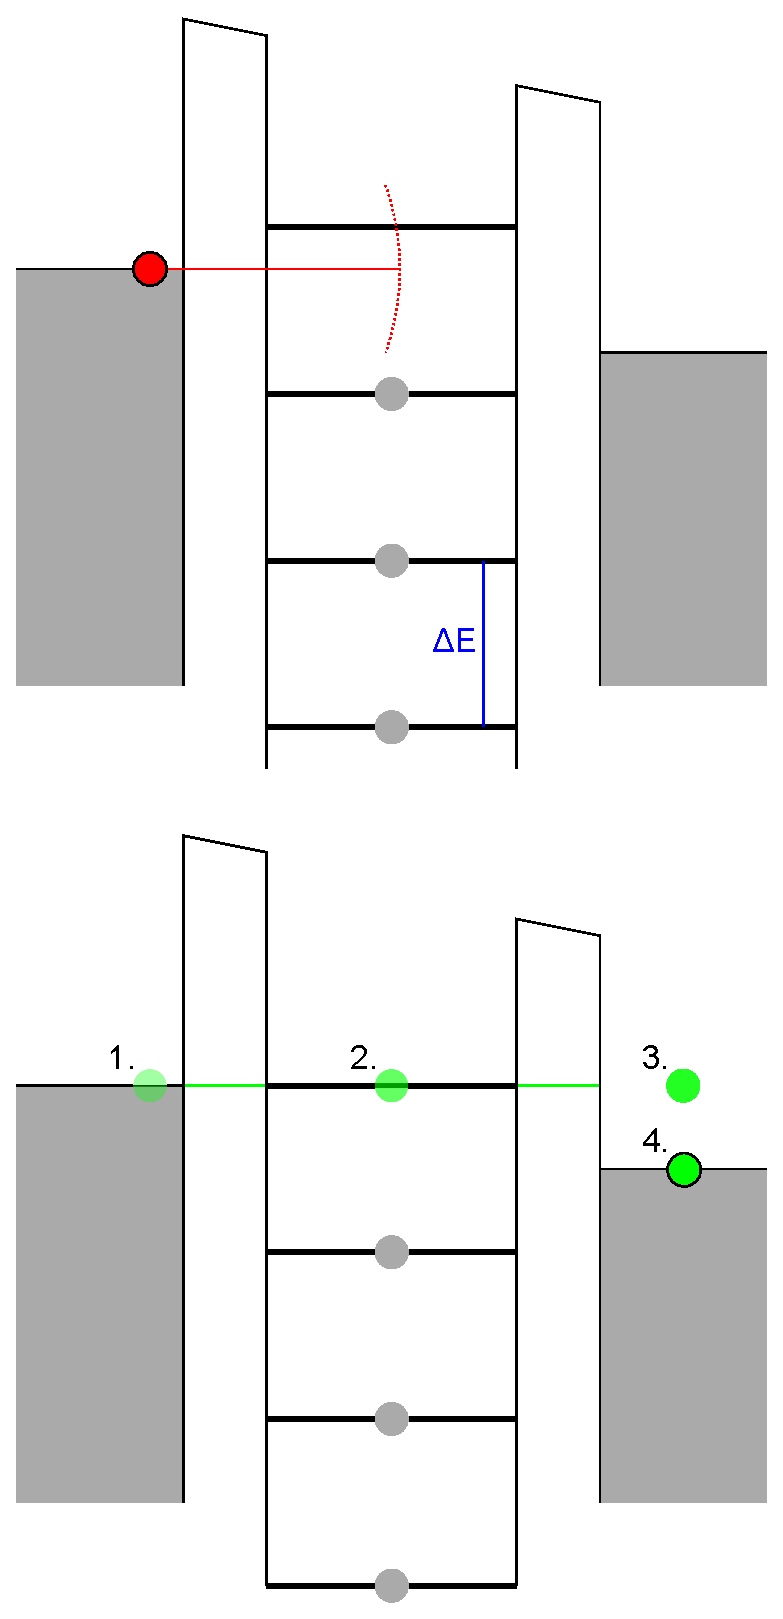
\includegraphics[width=0.6\textwidth, height=0.8\textheight]{coulomb_blockade}
	\caption{A Coulomb Blockade \cite{coulomb_blockade} forms due to electrostatic potential difference between island and source.\\ In the upper diagram, all allowable energy states are below the Fermi energy of the reservoir, hence no transmission can occur.\\ In the lower diagram, the potential of the quantum well has been raised, and now an empty state can be occupied by an electron from the source, which will subsequently tunnel off to the drain.}
	\label{coulomb_blockade}
\end{figure}

\begin{figure}[htbp!]
	\centering
	\includegraphics[width=0.8\textwidth]{coulomb_peaks}
	\caption{Coulomb Peaks form due to the discrete energy levels allowed on the island}
	\label{fig::coulomb_peaks}
\end{figure}



\cite{nuclear_spin_readout}


\cite{bonato2015optimized}
\subsection{Devices}
\subsubsection{PCIe Digitizer Card}
\todo[inline]{Talking points of the Digitizer solution, DMA, etc. etc.}
\cite{ATS9440}
%\subsubsection{FPGA/$\mu$Controller and ADC}
\todo[inline]{Talking points of the external FPGA and ADC solution, mention some particular examples of ADCs etc.}
\subsubsection{XMC}
\todo[inline]{Talking points of the integrated XMC solution, pre-built FPGA, ADCs and possibly with Auto-DMA}

\pagebreak
\section{Simulation}
\label{sec::simulation}
\subsection{Post-Processing Results}
	To verify MATLAB as a viable solution, it was first used against a full set of data that had been collected from a previous experiment. A set of 3 tests were performed, the first was to simply process the entire data in a single operation. This was the least like a real-world test, but served as a proof of concept that the peak detection, and time-out period were working. Once this was established, the next logical step was to perform this task on subsets, or windows, of the full data set. This is closer to a real test, and is actually extensible to the next alternative solution, as data processing on an embedded system can be limited by available memory. The test itself performed as expected, mirroring the first test. The final test was perhaps the most like a real-world solution, where a circular buffer of a fixed size (512 samples) is filled, which mimics a streaming input. This allows for a near-real-time time-out detection, supposing that the time it takes to process the signal is less than the time it takes to fill a time slice of the buffer (arbitrary, 32 samples in this example). Figure \ref{fig::timeout_detection} depicts the windowed solution in action over a large data set.
	
	\begin{figure}[htbp!]
		\centering
		\includegraphics[width=\textwidth]{timeout_detection}
		\caption[MATLAB windowed peak detection on generated data]{MATLAB performing peak detection on windows of the green data set. The blue dashed line represents the output signal, once a set amount of time has passed}
		\label{fig::timeout_detection}
	\end{figure}

\pagebreak
\section{Real-time Processing}
\subsection{Device under Test}
\label{sec::experiment}
\todo[inline]{Replace this section with Berdina}
Though experiments and designs are constantly evolving, at the core of this group's research is an \gls{set} used to perform electron spin readout. The apparatus I am applying my work to is by no means comprehensive, but it serves as a reference point in a proven device \cite{morello2010single}. To improve spin initialisation with this particular device would therefore be extensible to other devices and experiments.
Figure \ref{fig::thesis_experiment} shows a general layout used to control and read from an \gls{set}.

\begin{figure}[htbp!]
	\centering
	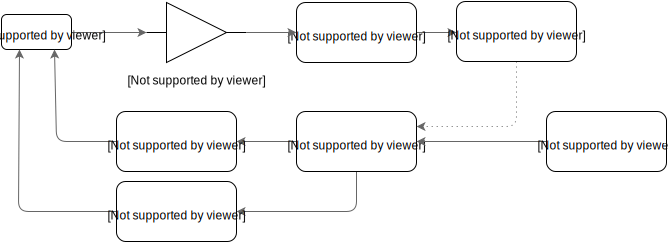
\includegraphics[width=\textwidth]{thesis_experiment.pdf}
	\caption{Block diagram of experiment}
	\label{fig::thesis_experiment}
\end{figure}


Figure \ref{fig::set_layout} shows the physical device that will be similar to one I will be testing my solution on. This devices has various voltage-controlled nodes, such as the top gate to induce a layer of electrons on the boundary, the left and right barriers to remove this layer, forming tunnel junctions to the island, and finally the plunger which can act at the gate as defined in section \ref{sec::set}.

\begin{figure}[htbp!]
	\centering
	\includegraphics[width=\textwidth]{set_layout}
	\caption[Layout of an \gls{set}]{The layout of an \gls{set}\cite{morello2010single}}
	\label{fig::set_layout}
\end{figure}

\subsection{Problem Statement}
The problem with this current approach is the cost of running these experiments if at the point of the plunge there was no electron on the donor. Any data with an incorrect initialization must be discarded, so as not to disturb the results. To take this one step further, to require 99.9\% spin-down initialization fidelity would mean ignoring over 90\% of all recorded data. This kind of waste can be circumvented by a feedback loop that can decide when the initialization has been performed correctly, and thus continue the experiment.

The problem I am to solve in this thesis is to incorporate digital feedback with current research, closing the loop in Figure \ref{fig::thesis_experiment}, which will allow for experiments to run more efficiently and lessen the burden on the researchers in selecting their data. The following section will detail some available solutions.

\subsection{Process}

	\subsubsection{Electrostatic Stimulus}
	\todo[inline]{discuss gate tuning, explain here or earlier how the fermi level/donor level is shifted by applying a voltage}
	\todo[inline]{Add pulse sequence explanation here}
	To allow for precise control and measurement of the steering time applied to the electron donor, an electrostatic environment needed to be defined, along with radio and microwave stimulus. The SET donor is coupled capacitively to a number of gates.
	
\pagebreak
\section{Results}
\subsection{Nuclear Spin Mapping Fidelity}
\todo[inline]{Discuss all results related to nuclear spin mapping}

	As discussed earlier\todo{cite section}, nuclear spin mapping was used to improve the readout fidelity of our experiment. However, the improvement in fidelity was conditional upon the initial state of the electron at the time of the mapping. To perform correct mapping, a spin-down electron is required. Figure \ref{fig::wait_time} shows the total experimental error as a function of steering time. As steering time increases, we are more confident that the state of the electron was spin-down at the time of mapping, which is reflected in our decrease in error. The average time spent in the initialisation period is plotted on the right-axis. This would exceed the steering time in the average case, as a blip in current would require postponement of the donor plunge.
	\begin{figure}[htbp!]
		\centering
		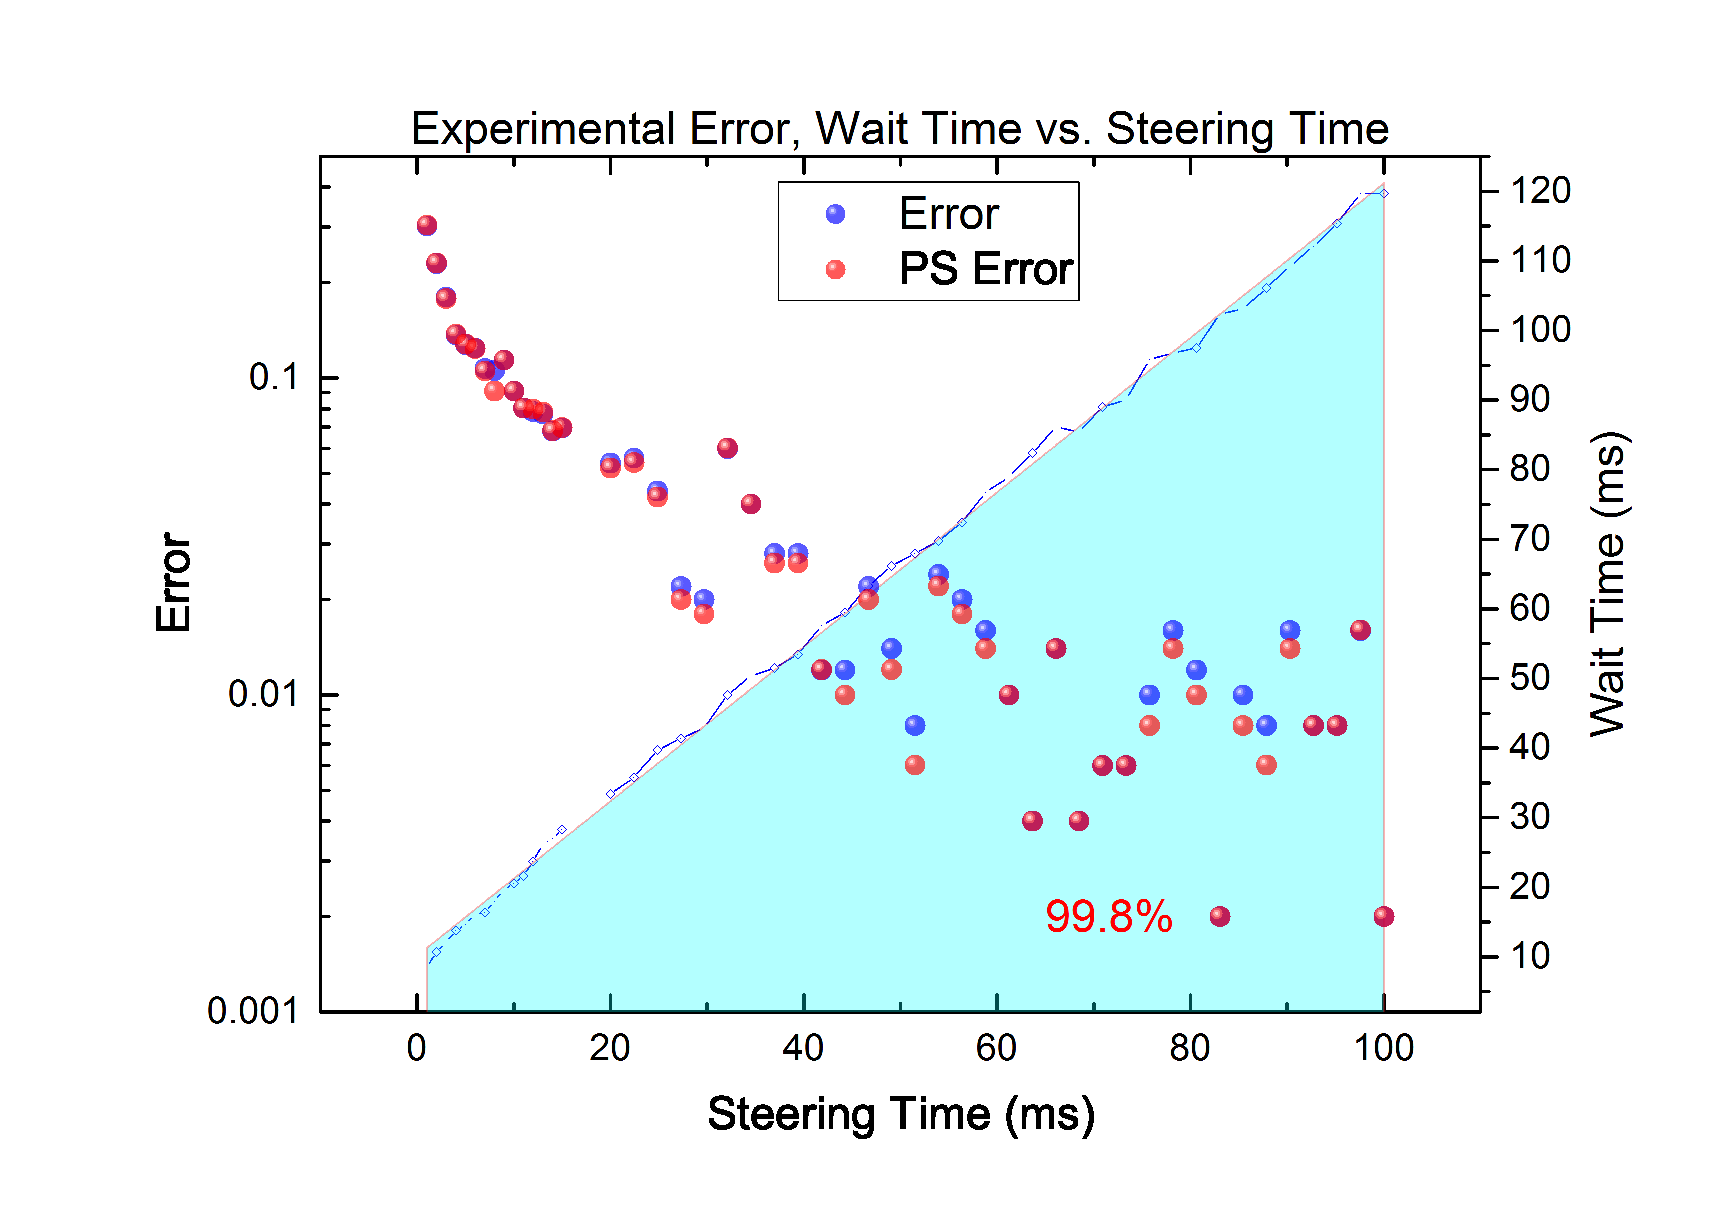
\includegraphics[width=0.8\textwidth]{WaitTimeFigLog}
		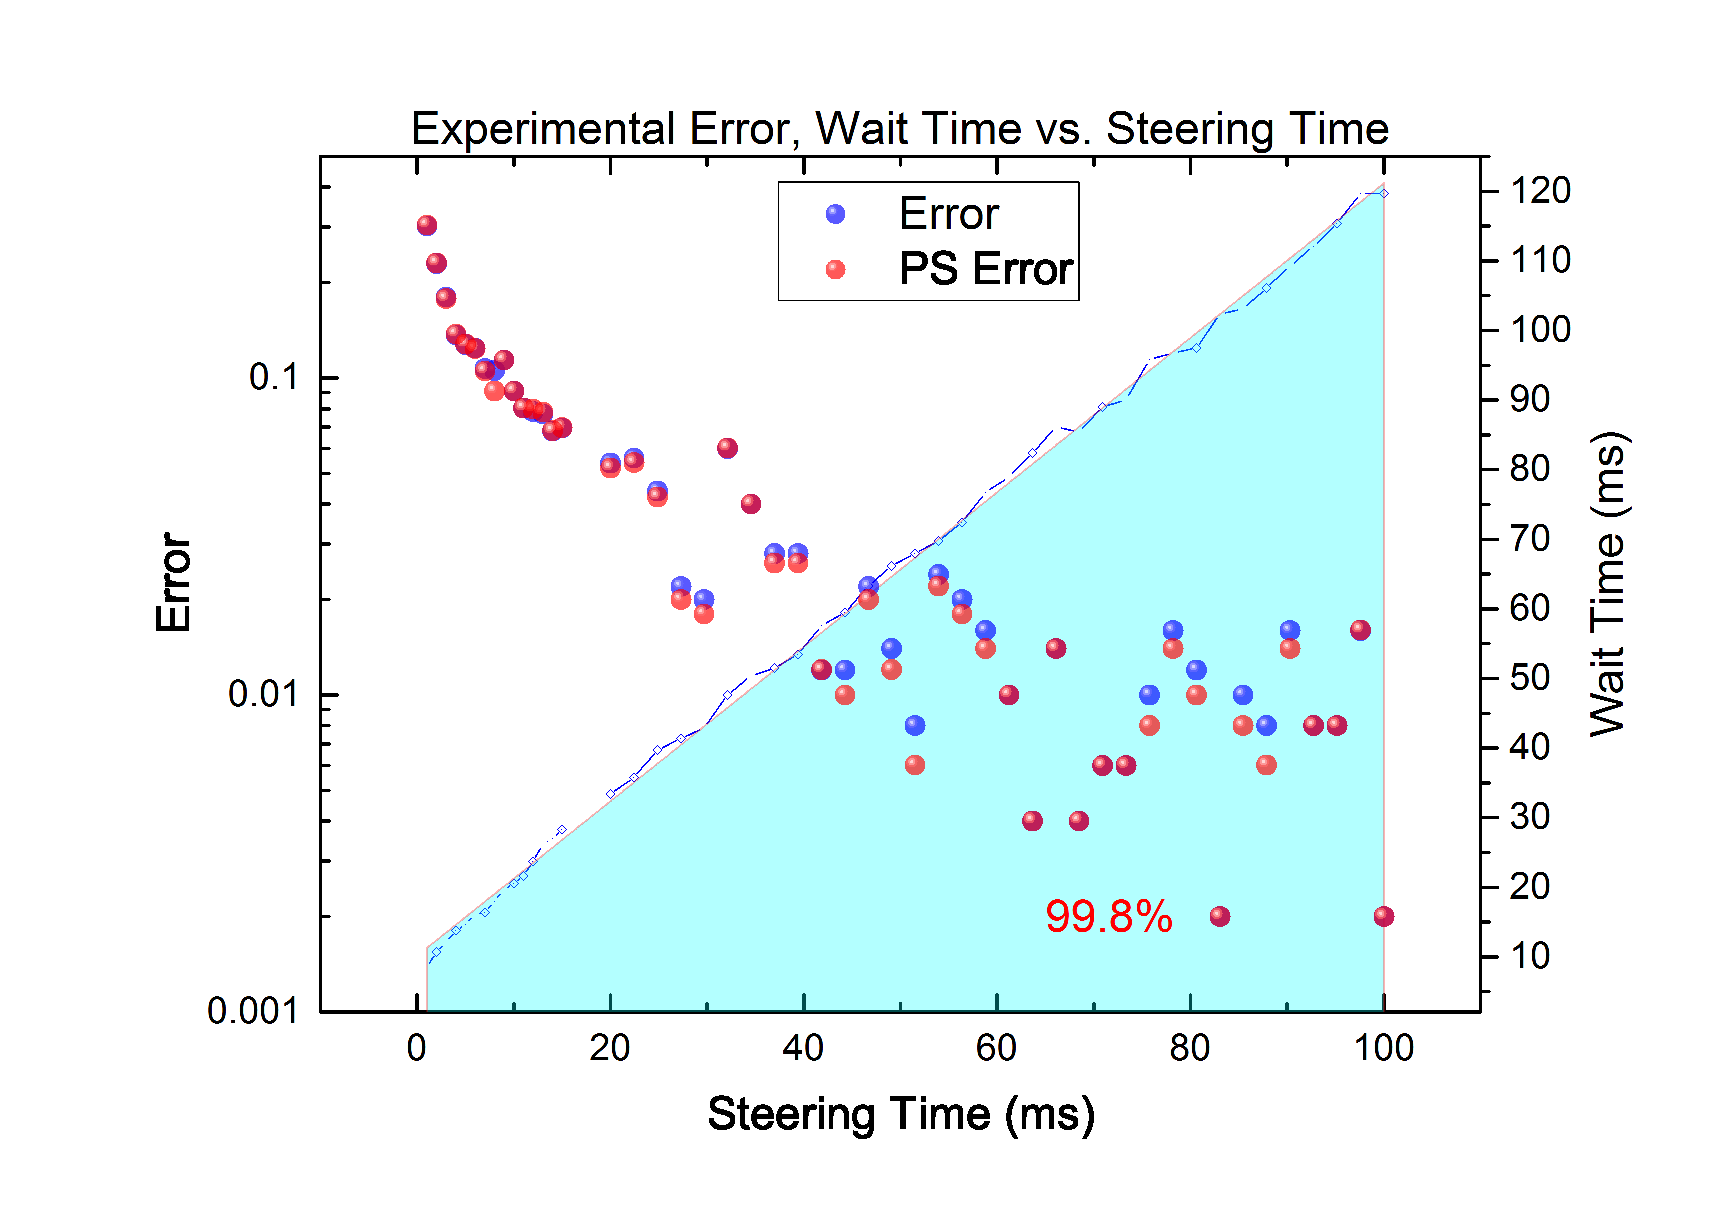
\includegraphics[width=0.8\textwidth]{WaitTimeFigLog}
		\caption{For a field of $B = 1.4$ T (top) and $B = 1.0$ T (bottom), the experimental error is plotted against steering time. On  the right axis is the average time spent at the initialisation level during the experiment.}
		\label{fig::wait_time}
	\end{figure}
	
	There are 2 separate data sets plotted, one for $B = 1.4$ T and the other for $B = 1$ T. These two datasets show the relationship between the required steering time for a good initialisation and the apparent tunnelling time of the donor electron. The required steering time to achieve 99\% fidelity is much longer for $B = 1$ T, however it was observed that the average tunnel time had not increased by such a margin from $B = 1.4$ T. This could be explained if we accept that the probability of a spin-down electron tunnelling off during the initialisation phase is high (also known as a dark-count), which is equivalent to a read-error. Whilst this is a possible explanation, it's not clear if this is accurate, and more examination of the data is required.

\subsection{Nuclear and Electron Rabi Oscillations}
	\todo[inline]{Discuss results pertaining to a high fidelity readout from a nuclear/electron rabi}
	Figure \ref{fig::nuclear_rabi} show a demonstration of the improvement that can be achieved using this initialisation scheme.
	
	The generic nuclear Rabi oscillation was performed by loading an electron onto the donor, followed my mapping the state onto the nucleus. This electron is ideally spin-down for this step. After the nucleus is prepared, we stimulate it with a \gls{rf} pulse of duration $\tau_{RF}$, which is swept as part of the experiment. After the \gls{rf} exposure, we then map the nucleus state back onto an electron using another \gls{mw} pulse, followed by a readout of the electron state. We perform 20 repeated measures of the nuclear state via the electron in this manner.
	
	As we vary $\tau_{RF}$, we observe that the expected value of the nuclear-spin readout, via the electron readout, follows a sinusoid with a frequency known as the Rabi frequency. Arbitrary rotations are a key part of a quantum system, and naturally improving the initialisation fidelity can allow for finer rotations.
	
	\begin{figure}[H]
		\centering
		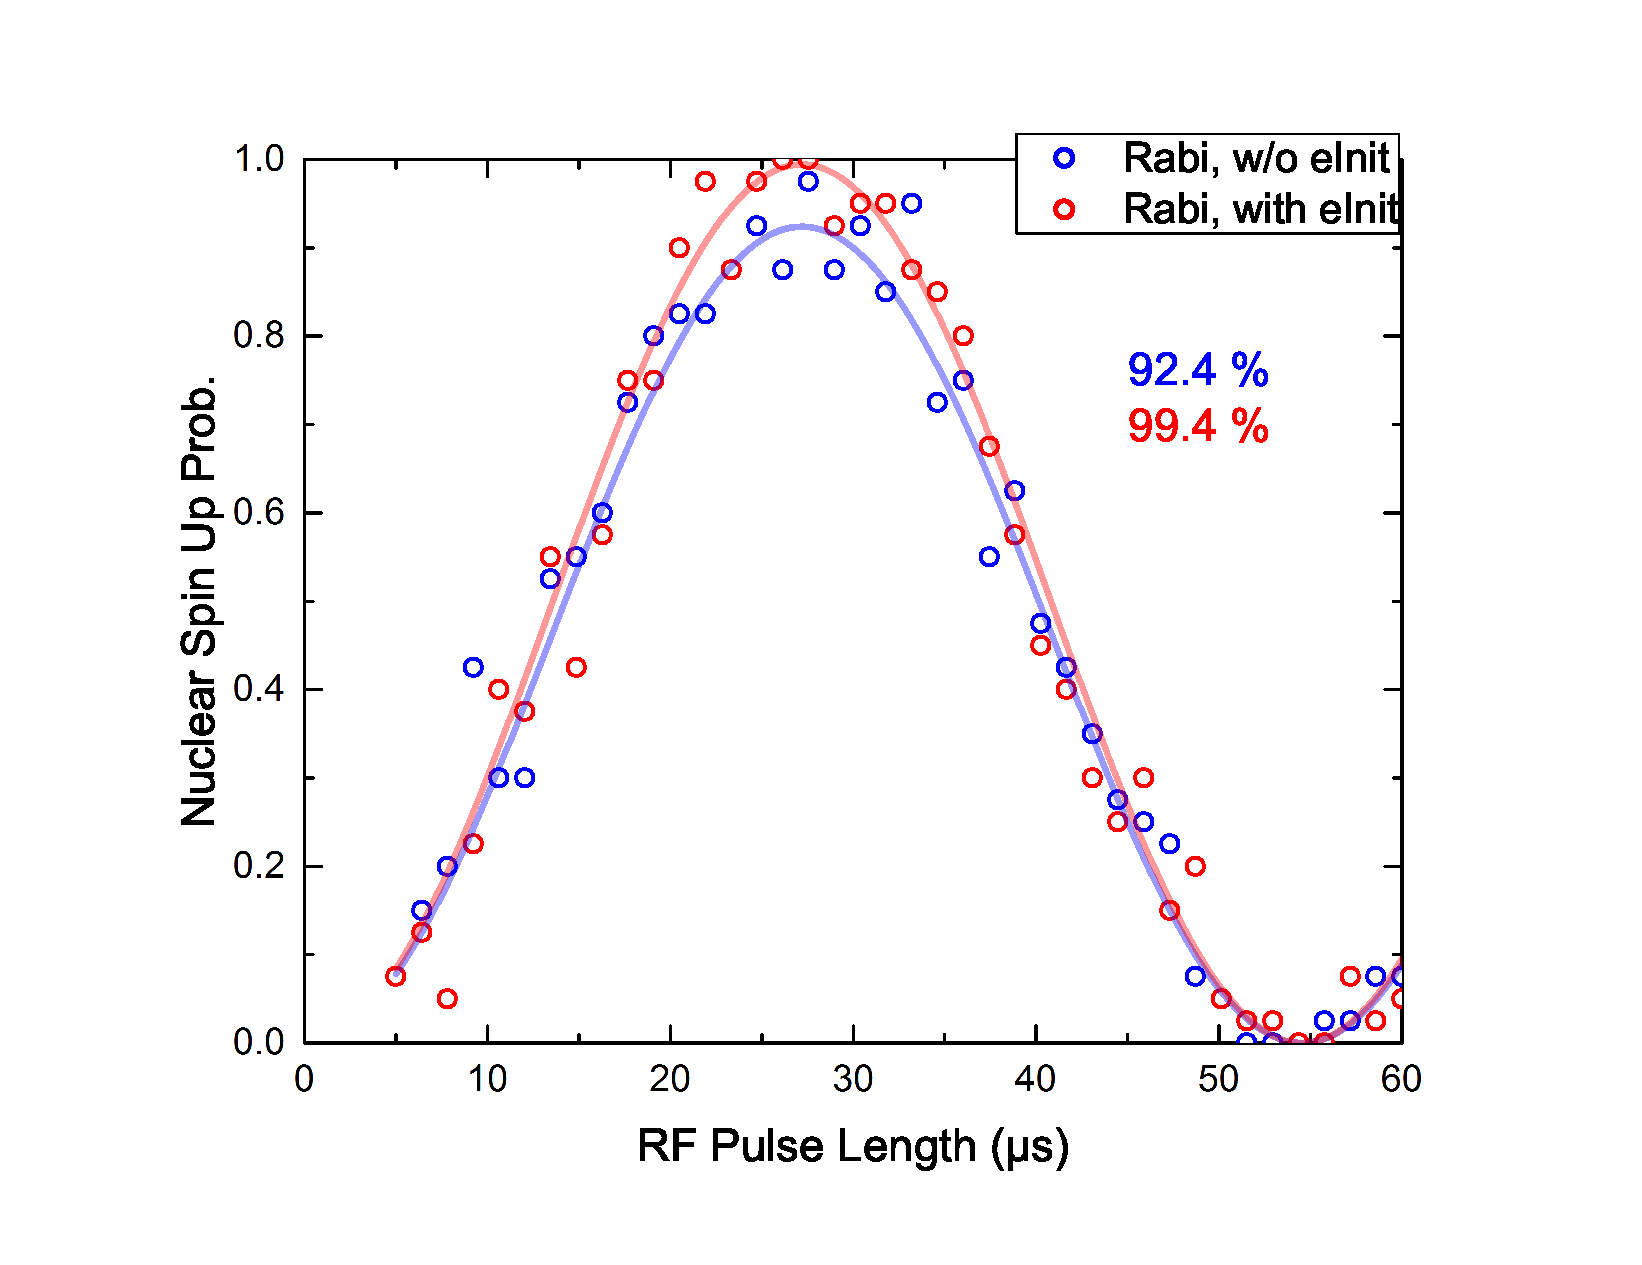
\includegraphics[width=0.8\textwidth]{nRabiFig}
		\caption{A nuclear Rabi oscillation with and without electron intialisation.}
		\label{fig::nuclear_rabi}
	\end{figure}
	
	If we have poor initialisation, this will affect the fidelity of our readout and would reduce the height of the peaks, as shown by the maximum of the fitted sinewave reaching only 92.4\% without intialisation, compared to 99.4\% with intialisation.

\subsection{Initialisation Level Tuning}
	The initialisation level of the pulse sequence was tuned to find the best position for a high fidelity experiment. It was discovered, however, that with initialisation there was a broad (approximately 400 mV) flat-band in which high fidelity results were obtained. This indicates another benefit in performing electron initialisation, which is insensitivity to tuning. This is a very useful property for a quantum computer, as reproducibility of measurements is crucial in determining the result of a computation.
%	
	\begin{figure}[htbp!]
		\flushleft
		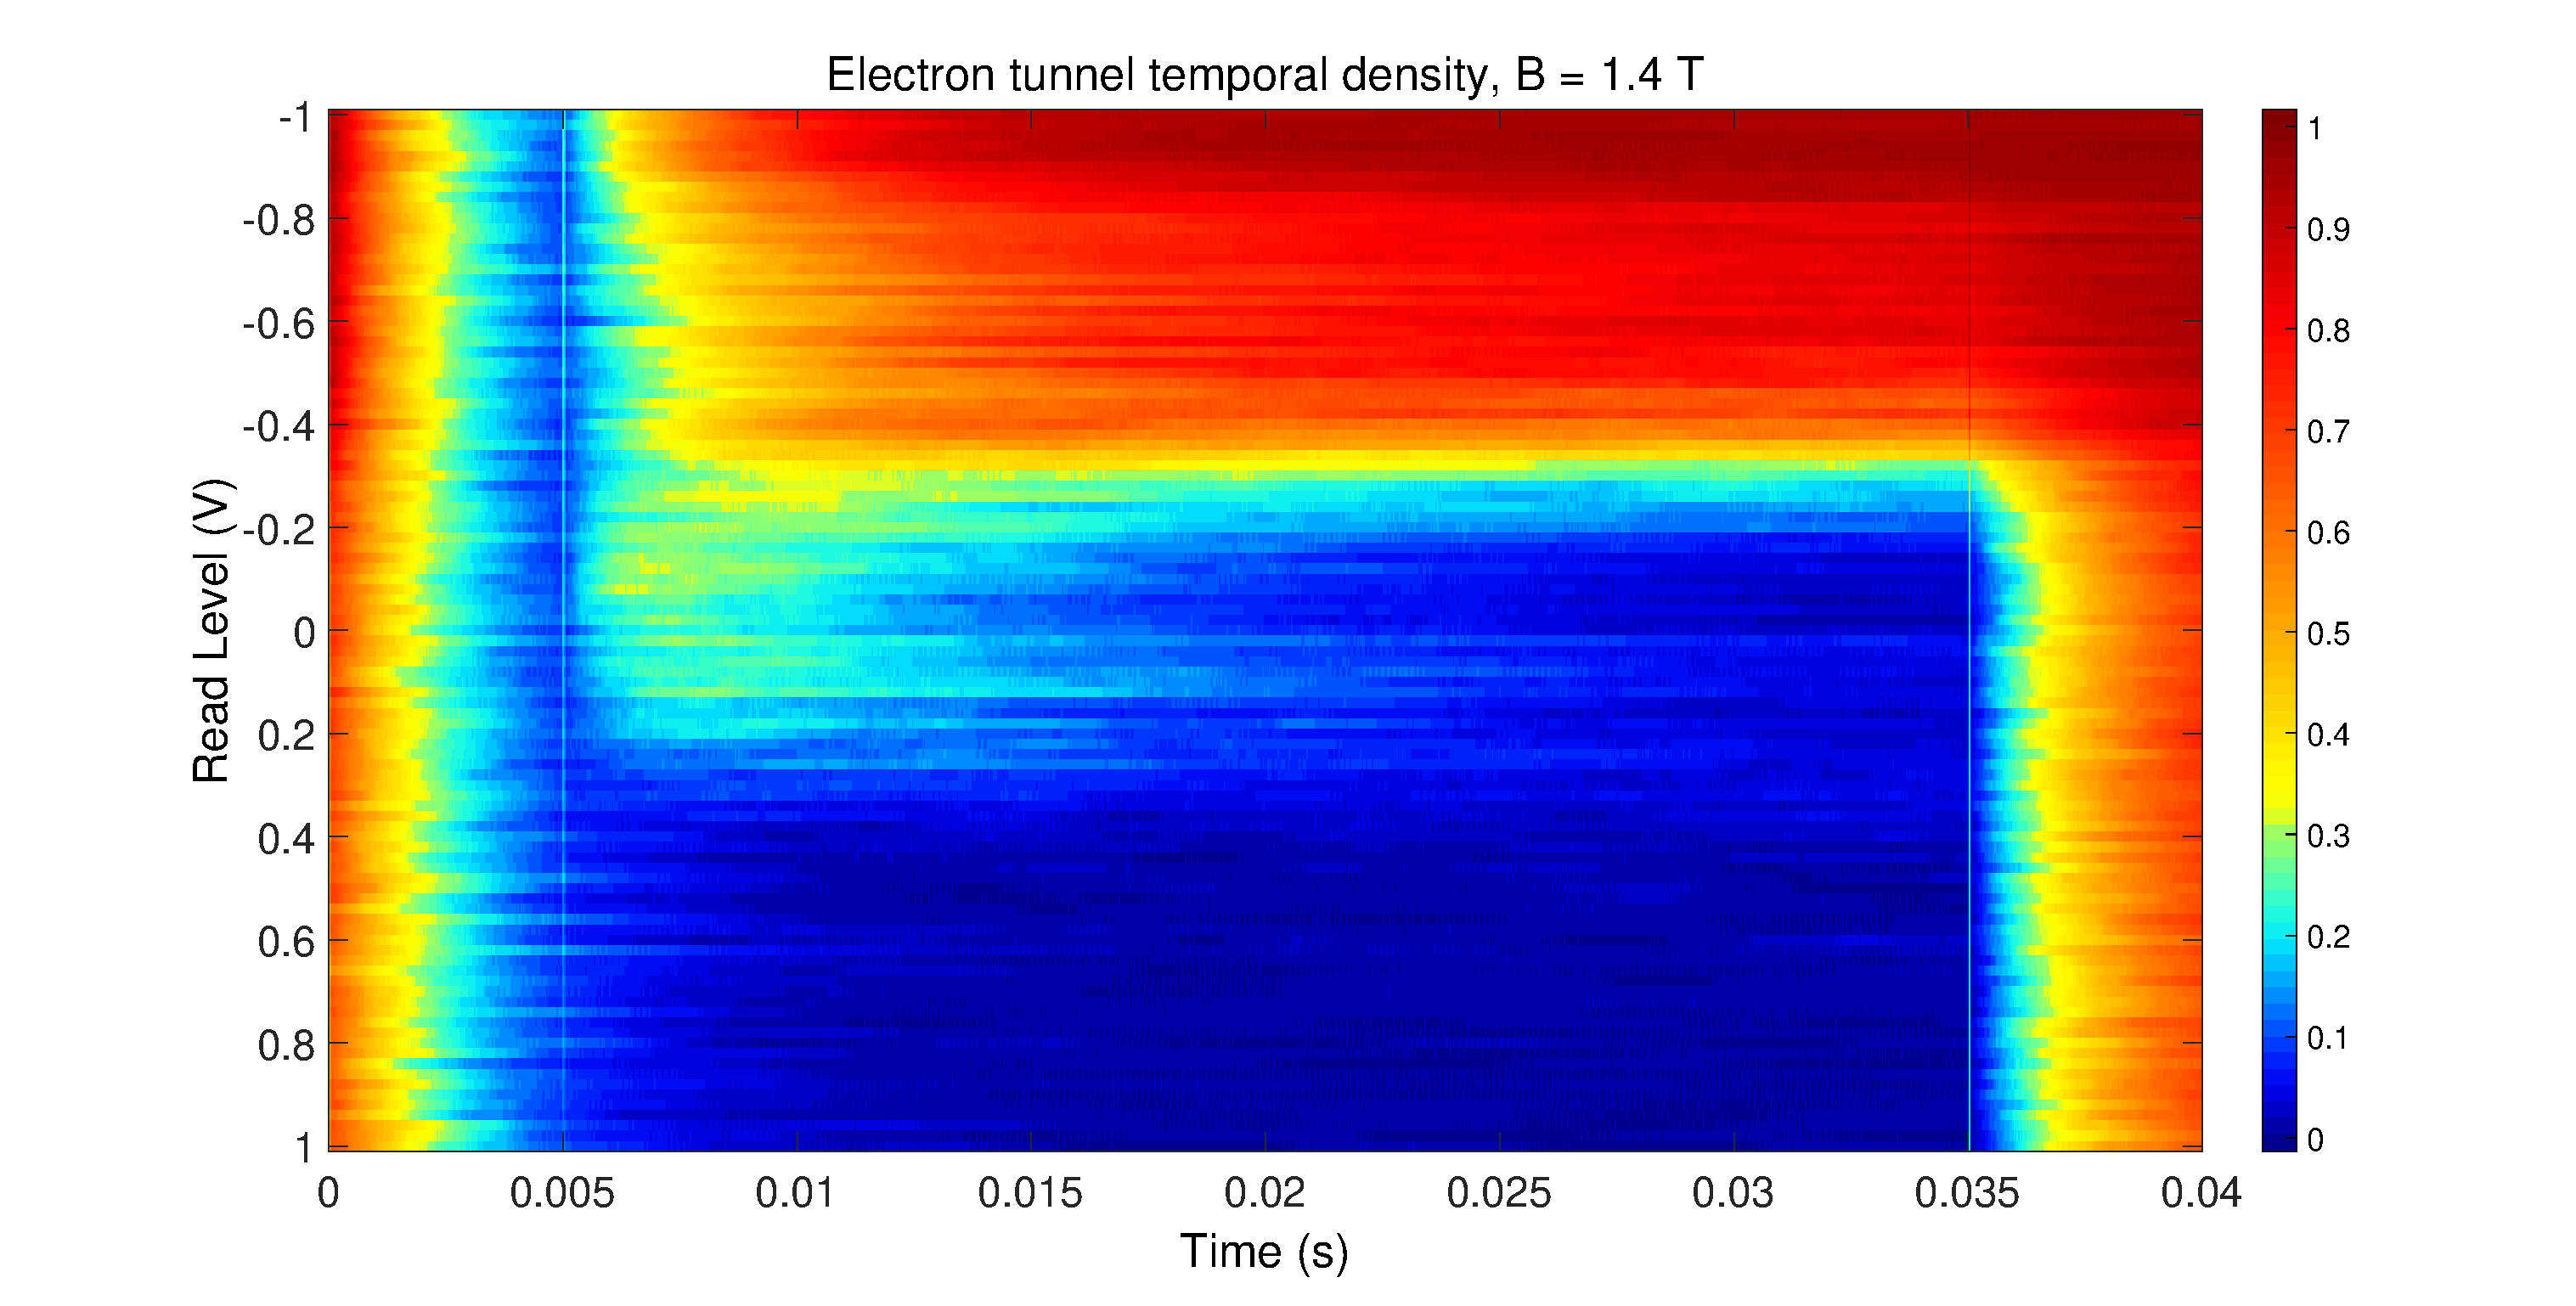
\includegraphics[width=\textwidth]{readLevelScan_1p4T}
		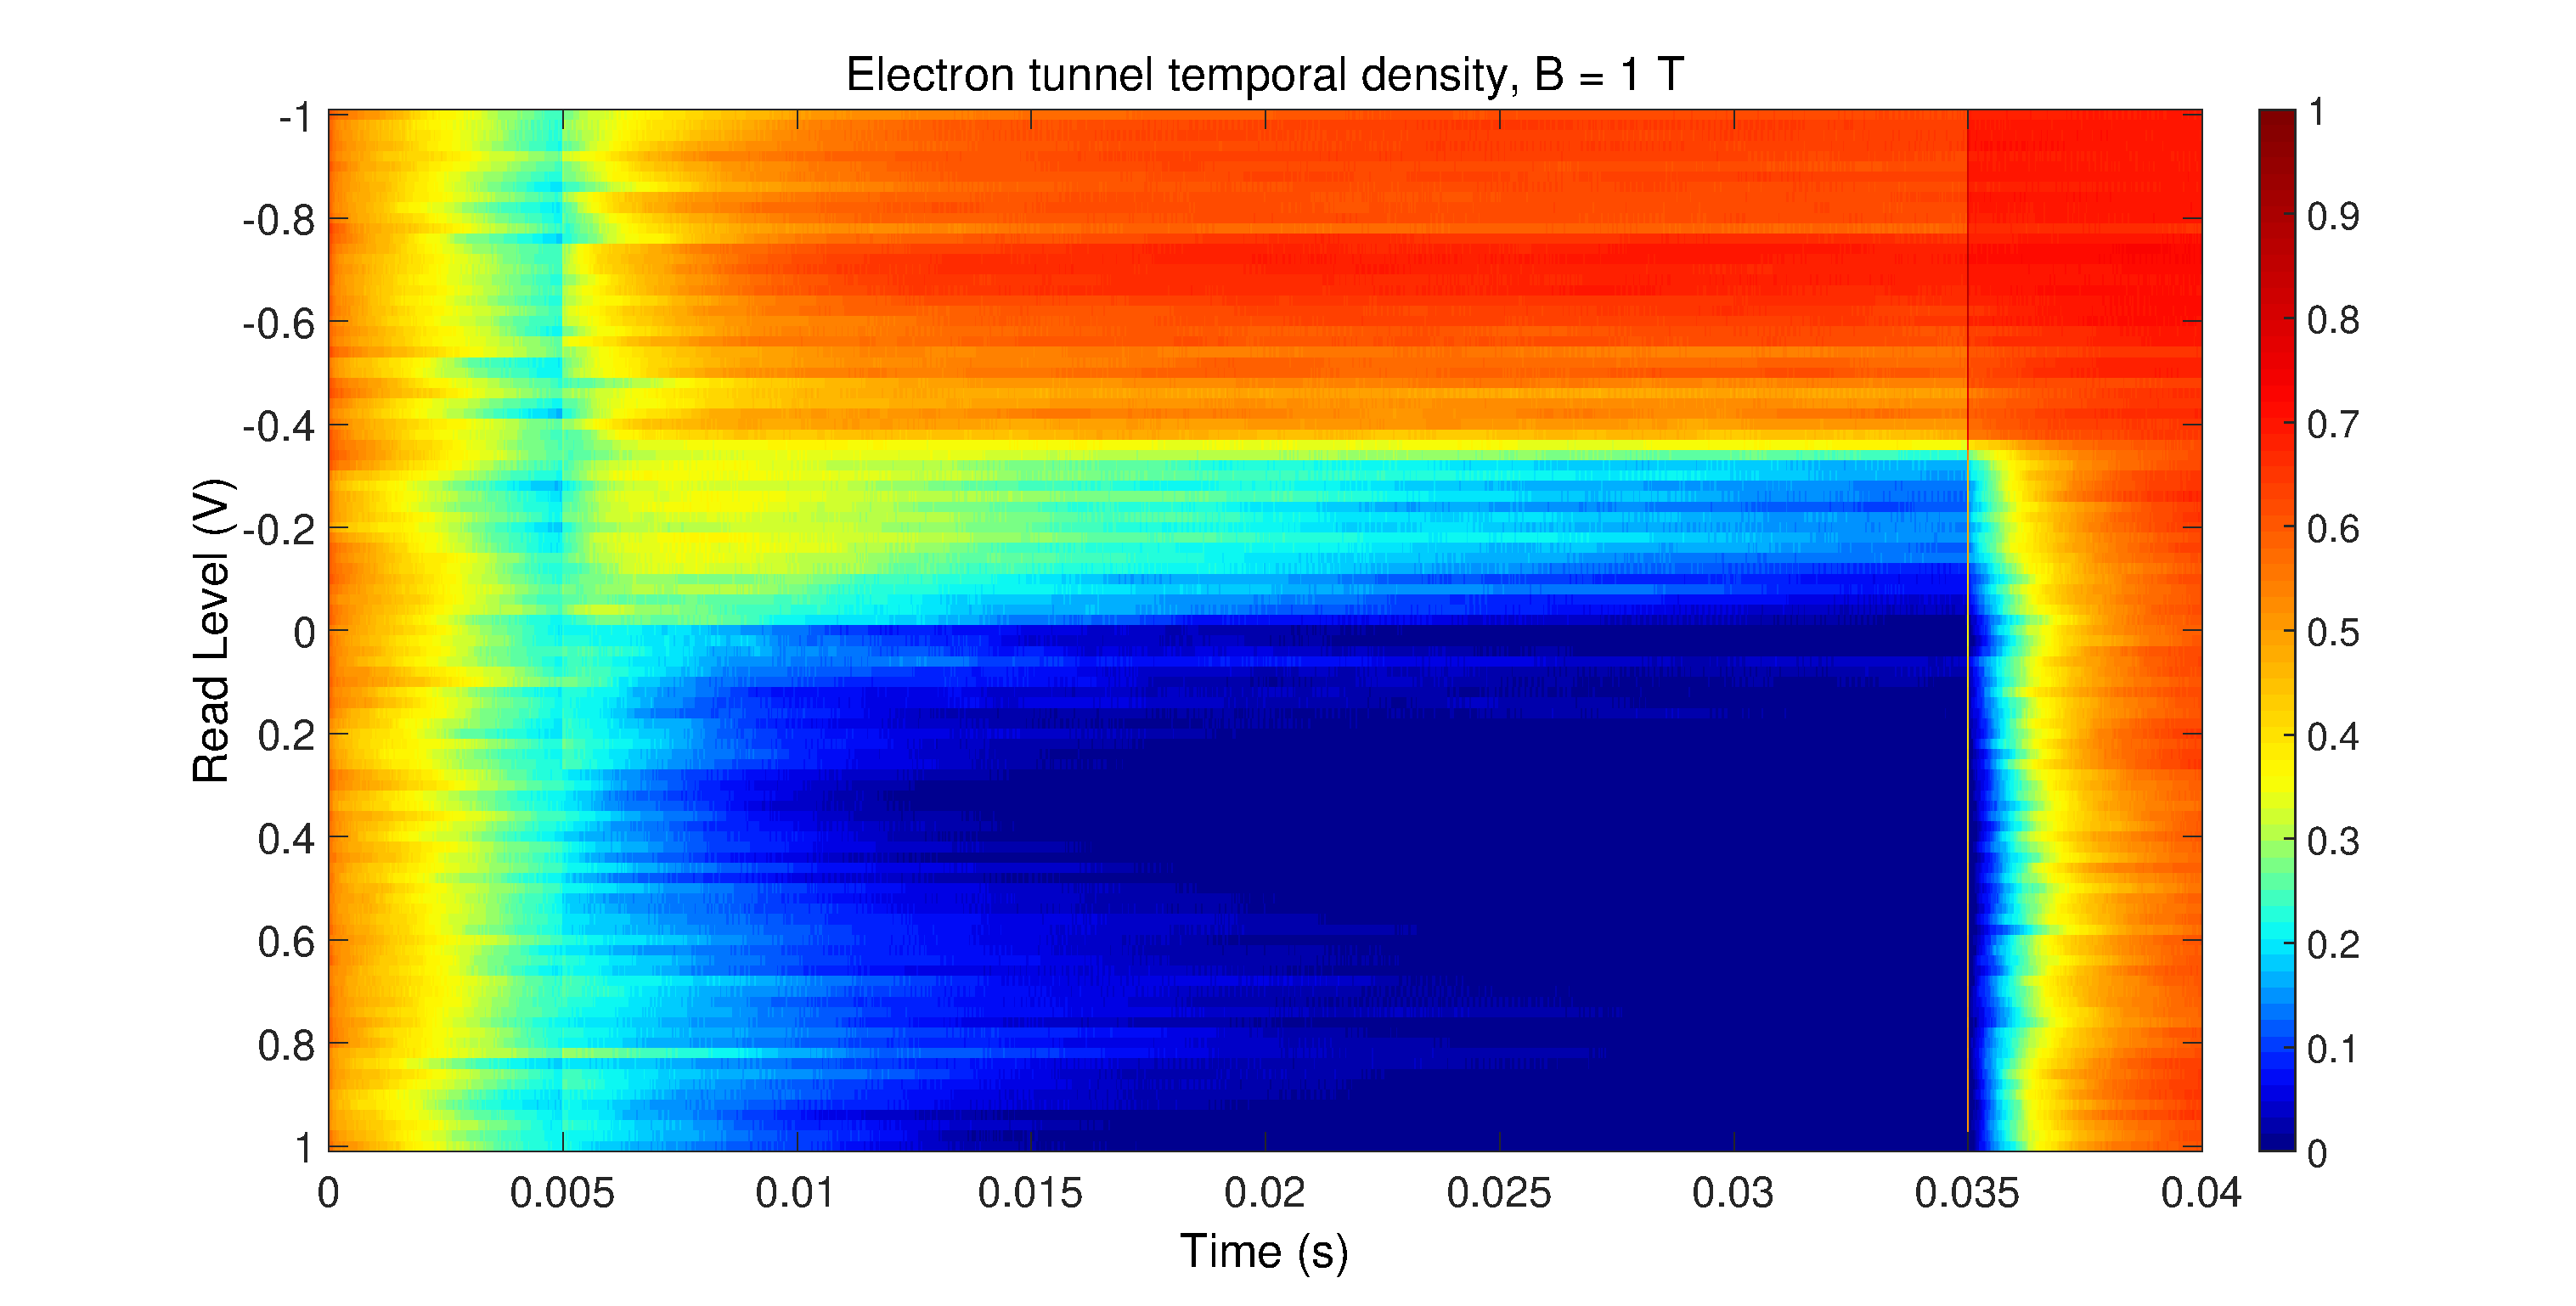
\includegraphics[width=\textwidth]{readLevelScan_1p0T}
		\caption{For a field of $B = 1.4$ T (top) and $B = 1.0$ T (bottom), the tail of a read level scan is plotted.}
	\end{figure}
	
	Another novel application of this measurement is that we can infer the donor temperature from the width of the flat-band. The flat-band itself is a measure of the tail reading from the Zeeman splitting of the electron donor, assuming finite temperature.


\pagebreak
\section{Design Improvements}
To improve further on initialisation, this software-defined feedback loop should be shifted into an integrated solution, such as a purpose-built solution with a \gls{mcu} or \gls{fpga}. While an \gls{fpga} would be easy to apply to the problem of detecting blips and measuring time, there is a complexity in integrating an \gls{fpga} based solution with \gls{daq}. 

Data acquisition has been solely performed by a \gls{pcie} connected digitizer card, where data is dumped directly to memory and then saved to a hard-disk. If an \gls{fpga} were to be used in the manner described above, it would either need to introduce a separate \gls{daq} system, where data processed in the \gls{fpga} is collected separately from what is stored on hard-disk, or the introduced \gls{daq} would need to also store its data for analysis.

\begin{figure}[htbp]
	\centering
	\includegraphics[width=\textwidth]{thesis_redesign_1}
	\caption{An integrated solution which writes data back to disk.}
	\label{fig::redesign_1}
\end{figure}

The first solution holds far more complexity, as it requires designing a system with a \gls{daq} and an \gls{fpga}. This would likely end up using a custom \gls{pcb}, with a special purpose \gls{adc}. The construction and verification of such a device is an undertaking not suited for a research environment where this is not the end product. Similarly, the second solution is not ideal. Storing data from an \gls{fpga} would again require specialised hardware to interface with a hard-disk. 


\begin{figure}[htbp]
	\centering
	\includegraphics[width=\textwidth]{thesis_redesign_2}
	\caption{An integrated solution which adds a separate data acquisition stage to the feedback loop.}
	\label{fig::redesign_2}
\end{figure}

Ultimately, the desired solution should be integrated in a manner fit for use by non-electronic specialists. As such, a rework of the current set-up will be the preferred method of achieving real-time digital feedback.

The proposed solution is to utilise a \gls{pxie} cabinet with multiple slots to integrate the varied signals and sources we use, including an \gls{awg} and a \gls{daq}. For the problem at hand, there exist combination \gls{fpga} and \gls{daq} cards that allow for pre-processing data and controlling a single digital output, or in more advanced devices, controlling an \gls{awg} via the \gls{fpga}. This solution will be sufficient for performing threshold analysis on a single channel, however it does not make the most of the advantage an \gls{fpga} has over a \gls{mcu}. It has been shown internally in an unpublished form that a \gls{dwt} can detect blips that occur below the threshold level, due to the finite bandwidth of the device and sampling rate of the \gls{daq}.

A Haar \gls{dwt} was used in post-processing data to yield a high-fidelity readout. If this is combined with the initialisation scheme defined in this report, total experiment fidelity is expected to increase much further for lower steering times, and ultimately be more reliable. It would also allow the amplifier bandwidth to be opened up, as the increase in noise will be filtered by the transform. \gls{dwt} implementations in hardware \cite{PeiYinChen2004,hsieh2006novel,Salama2006} are commonplace, and highlight the validity and potential of an integrated \gls{fpga} based solution to the problem assessed in this thesis. 



\pagebreak
%\section{Prospective Results}
%\todo[inline]{try and get some simulation results using teh Haar wavelet transform, showing the algorithm run time/latency}
%\pagebreak
\section{Conclusion}
\todo[inline]{Conclude, like normal}
\pagebreak

\bibliographystyle{ieeetr}	%IEEE style referencing
\bibliography{./src/references}
\pagebreak
\begin{appendices} 
	\section{Glossary}
	\printglossaries
	\pagebreak
	\section{Supplementary Information}
	\paragraph{Big O Notation} describes the limiting behaviour of a function when the argument tends toward infinity.
\label{supp::big_o}
For example, the leading term ($3 x^4$) in the polynomial $p(x) = 3 x^4 + 20 x^2 + 1$, represents the strongest factor that determines the behaviour of the function. As such, we say $p$ has order $\mathcal{O}(n^4)$. Note that we drop any constant multiplier as it doesn't modify the growth or shape of the function.
	\section{MATLAB Software Highlight}
	\lstinputlisting[breaklines=true, language=MATLAB,
					 basicstyle=\footnotesize\ttfamily,
					 numbers=left					
					]{./src/code_digitizer}
\end{appendices}
\end{document}
